\chapter{API Contracts Construction with Static Code Analysis}
\label{cha:codeAnalysis}
This chapter explains the concept of constructing caveat contracts from API caveats. In particular, it provides an overview of how caveat sentences from the Java 12 API documentation can be used to construct coding rules that are similar to code contracts, which can then be used in a static code analysis context to detect bugs in real-time.\\

\noindent
Section \ref{sec:contract-intro} provides background information for code contracts and an overview of the work conducted for this Chapter: constructing code contracts from API caveat sentences and using static code analysis to apply the contracts to code in real time. \\

\noindent
Section \ref{sec:contract-design} describes the design framework for generating and using code contracts. This includes a statistical analysis on the Java 12 API caveats, a description of the idea used for extracting information from caveat sentences for code contracts construction, and the concept of checker programs that can utilise the code contracts. \\

\noindent
Section \ref{sec:contract-implement} explains the implementation of API contracts construction and static code analysis in an IntelliJ proof-of-concept plugin. \\

\noindent
Section \ref{sec:contract-results} showcases the IntelliJ plugin developed that uses caveat contracts to detect API misuse. \fix{Extensions of this concept are also addressed.}

\section{Introduction}
\label{sec:contract-intro}
Code contracts are a concept derived from object-oriented principles in which preconditions, postconditions and invariants are defined for different software components. Specifically, the principle of ``design by contract'' suggests the use of specifications referred to as contracts. This provides a method for improving both code correctness and robustness as software components can only interact via obligations to contracts. Utilising this, we reduce the problem of linking API caveats to source code to the problem of mapping API caveats to code contracts, which we refer to as \textit{API caveat contracts} or simply \textit{caveat contracts} in this thesis. From this, we can improve understanding of API caveats considerably by providing real-time feedback during coding/development. Furthermore, finding a general method for transforming an arbitrary API caveat to a caveat contract is sufficient as we can assume the existence of programming analysis tools that can accept these contracts and locate patterns in source code (variations of such tools already exist). As a continuation of the previous chapter, I perform statistical analysis of several caveat types for the Java 12 API documentation based on work by \cite{zhou-directive}. I then propose a parsing technique to identify API caveats related to a significant subset of exceptions thrown and construct associated caveat contracts. This extends upon the parsing techniques used by \citeauthor{zhou-directive} to collect a subset of API caveats related to explicit constraints such as range limitations for arguments of a method, or not-null requirements. I propose and utilise an algorithm for analysing caveat sentences from this subset of API caveats to construct a total of 4,694 unique caveat contracts. Finally, I develop a proof-of-concept checker plugin for IntelliJ that can be used to highlight violations of these API contracts in real time. \\

\section{Design}
\label{sec:contract-design}
The first step to generating contracts for API caveats is the extraction of API caveat sentences as described in \ref{subsec:info-caveat-extract}. We recall that caveat extraction using the approach described by \cite{caveat-knowledge-graph} on the Java 12 reference documentation yields 
115,243 caveat sentences, where a significant proportion of the sentences (67,701) are found within miscellaneous sections of an API element such as sentences in the parameters section for a method, or the description of a methods return value. Furthermore, we note that a subset of API caveats dealing with directives \cite{zhou-directive} contain explicit constraints that represent the largest portion (43.7\%) of API documentation \cite{directives-study}. From \cite{zhou-directive}, it can also be seen that a set of heuristic rules can be used to obtain constraints of type: (1) nullness not allowed, (2) nullness allowed, (3) type restriction and (4) range limitation from the directives of an API document. Although other categories of API caveats can also potentially be transformed into contracts and applied to static code analysis, I focus primarily on the categories identified by \cite{zhou-directive} for the scope of this project. \\

In addition, \cite{code-examples} proposes a method for mining API misuse by transforming source code to structure they refer to as API call sequences. These sequences essentially capture an API method call in addition to surrounding code elements such as guard conditions and method calls that are most relevant to the target API call. From this, we note that caveat contracts can be modified to apply to API call sequences given that contracts can be transformed to a structure resembling API call sequences.

\begin{figure}
	\label{fig:contracct-architecture}
	\centering
	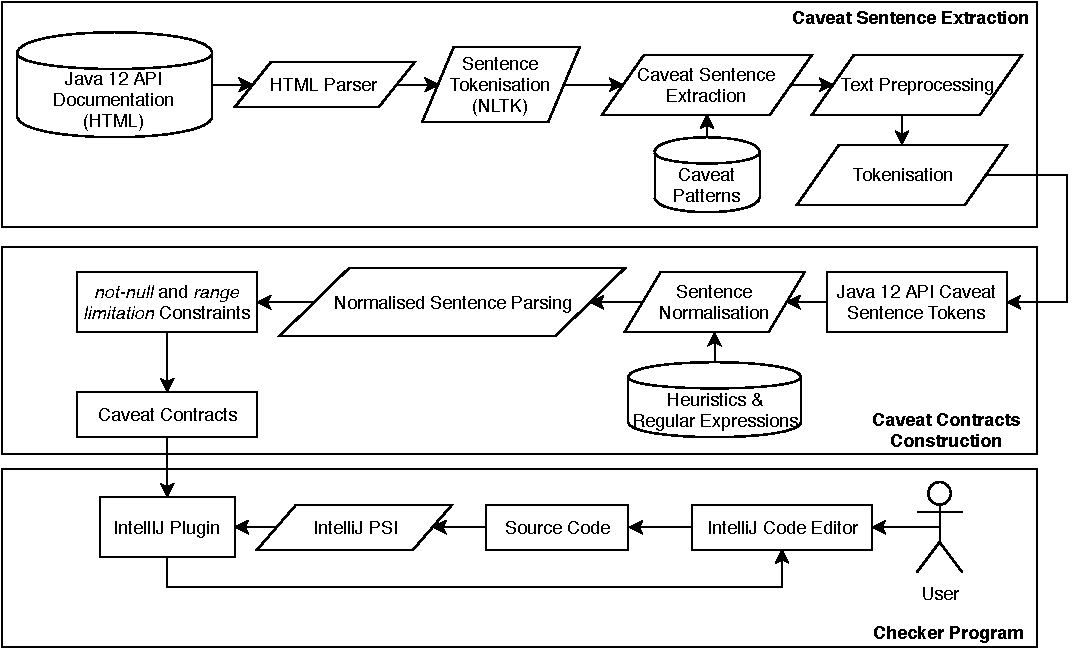
\includegraphics[width=0.8\textwidth]{figs/contract-architecture.pdf}
	\caption{Architecture design of the work for this chapter.}
\end{figure}

\subsection{Java 12 Caveat Statistics Analysis}
\label{subsec:contract-caveat-statistics}
To better understand the prevalence of these API caveat categories identified by \cite{zhou-directive} in the Java 12 documentation, a statistical sampling method from \cite{singh2013elements} is applied. Specifically, the minimum number of samples required to ensure the estimated population mean is within a given confidence level and error margin can be calculated by the formula:

\begin{equation}
\label{sample}
min=\frac{\frac{z^2\times 0.25}{e^2}}{1 + \frac{(\frac{z^2\times 0.25}{e^2} - 1)}{p}}
\end{equation}

Where $z$ is the z-score associated with the desired confidence level, $e$ is the error margin and $p$ is the population size. For a 95\% confidence interval, 5\% error margin and a population size of 115,243 caveat sentences, the minimum sample size is approximately 383. However, we observe that the directive constraints identified by \cite{zhou-directive} correspond to the parameter and exception sections of method API elements specifically. This is because the directives they analysed were sentences annotated with \textit{@param, exception} and \textit{@throws} tags within the comments of the JDK source code files, which are transformed into HTML via Javadoc. It is also noted that the heuristic rules formulated by the authors for caveat categories of not-null, nullness allowed, type restriction and range limitation are differentiated for sentences with the \textit{@param} tag and for sentences with either \textit{@exception} or \textit{@throws} tags. Thus, we adopt a similar approach to reduce the scope of caveat sentences that require analysis. We specifically focus on the parameter or exception sections only API methods and constructors, and regard the sentences from those sections separately. \\

An observation on the parameter and exception sections of the Java 12 documentation is the consistent structure used for sentences. Sentences form the parameter section follow a template of ``\verb|param - description|'', where \verb|param| is the name of the parameter for a given method/constructor and \verb|description| is the actual sentence describing some information about \verb|param|. Exceptions also follow a similar template of ``\verb|exception - description|'', where \verb|exception| is the exception class thrown and \verb|description| describes conditions required for the exception to be thrown. An example of this is shown in Figure \ref{fig:api-doc-charAt}. It is therefore trivial to separate the \verb|description| sub-parts of a caveat sentence for analysis as we are only interested on the constraints imposed upon a particular parameter and the exception conditions. Moreover, we can filter the corpus of exception and parameter sentences to obtain a unique set of sentences for both as identical sentences can be mapped to the same caveat contracts (but with different target parameters or API elements). Hence, two separate random samples of caveat sentences are collected: one from the parameters section of methods and constructors which consists of 2,654 unique sentences, and one from the exception sections of methods and constructors which consists of 4,870 unique sentences. Using equation \ref{sample}, the sample sizes required are 336 and 356 respectively. \\

\begin{figure}
	\label{fig:api-doc-charAt}
	\centering
	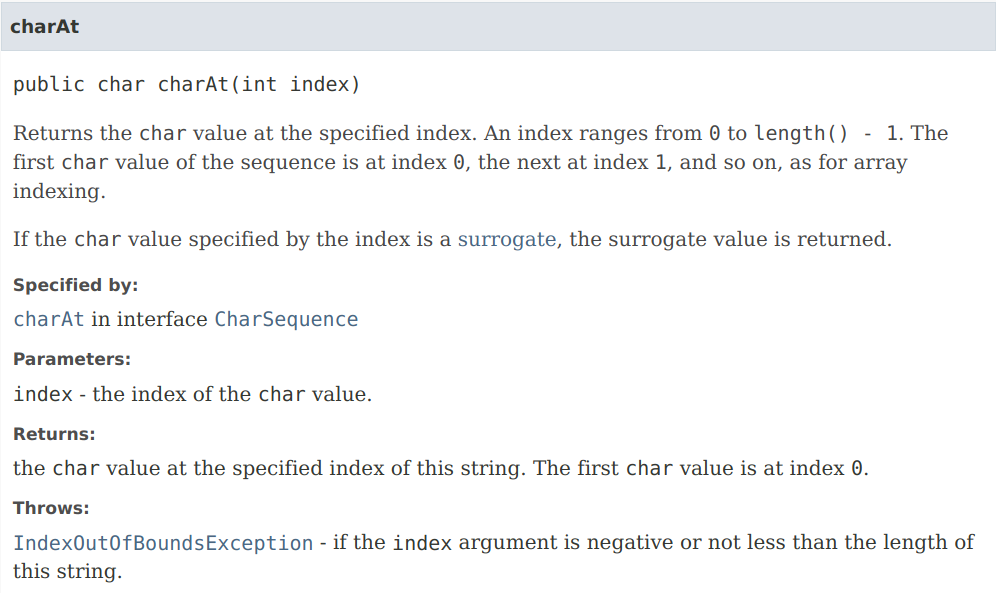
\includegraphics[width=0.75\textwidth]{figs/api-doc-charAt.png}
	\caption{API documentation for the \lstinline{charAt} method of the \lstinline{java.lang.String} class}
\end{figure}

Manual labelling is then required for the samples to identify the prevalence of different caveat types for the sentences. In  particular, the categories identified in \cite{zhou-directive} of \textit{not-null}, \textit{range limitation} and \textit{type restriction} are used as labels with the addition of \textit{ambiguous} to account for sentences that do not match any of the former classes. The \textit{not-null} category are defined as sentences which specify some parameter cannot be null. The \textit{range limitation} category specifies some numerical limitation on a parameter such as a non-negative requirement. Finally, the \textit{type restriction} category indicates that a parameter must a particular class type or one of several types. The \textit{nullness allowed} category is not considered from \cite{zhou-directive} because it only describes an acceptable condition for contracts, whereas the other categories describe a stricter condition for contracts that must not be broken. Overall, the results of this for the parameter sentences sample is shown in Table \ref{tab:caveat-param-stats}, while the results for exception level sentences is shown in Table \ref{tab:caveat-exception-stats}. We note that for \ref{tab:caveat-exception-stats}, the counts contribute add up to more than 356 because 6 of the labelled caveat samples fit both the \textit{not-null} category and the \textit{range limitation} category. 

\begin{table}[]
	\begin{tabular}{|l|cccc|}
		\hline
		& \multicolumn{4}{c|}{\textbf{Labels}} \\ \cline{2-5} 
		& \textbf{ambiguous} & \textbf{not-null} & \textbf{range limitation} & \textbf{type restriction} \\ \hline
		\textbf{Count} & 291 & 26 & 19 & 0 \\ \hline
	\end{tabular}
	\caption{Manually labelled results for classes of 336 randomly sampled parameter level caveat sentences.}
	\label{tab:caveat-param-stats}
\end{table}

\begin{table}[]
	\begin{tabular}{|l|cccc|}
		\hline
		& \multicolumn{4}{c|}{\textbf{Labels}} \\ \cline{2-5} 
		& \textbf{ambiguous} & \textbf{not-null} & \textbf{range limitation} & \textbf{type restriction} \\ \hline
		\textbf{Count} & 242 & 73 & 46 & 1 \\ \hline
	\end{tabular}
	\caption{Manually labelled results for classes of 356 randomly sampled exception level caveat sentences.}
	\label{tab:caveat-exception-stats}
\end{table}

From Table \ref{tab:caveat-param-stats}, it can be seen estimated that approximately 8\% of unique parameter caveat sentences impose a \textit{not-null} constraint and approximately 6\% of the unique parameter caveat sentences impose a \textit{range limitation} constraint. Despite the small percentage of sentences in parameter sentences sample that fit these categories, it its important to note that they represent one the most important type of API caveats: caveats that can cause software failures from exceptions. Furthermore, these caveat types are found to require (generally) explicit constraints that have little dependencies on other API elements, which makes them an adequate baseline for constructing caveat contracts. In contrast, the results from Table \ref{tab:caveat-exception-stats} show that considerably larger subset of 20\% of unique exception caveat sentences specify a \textit{non-null} constraint. This is also observed for the \textit{range limitation} category with approximately 13\% of sentences labelled. \\

Analysis of other categories must also be considered to determine what caveat contracts can be constructed and the approaches that are available. In particular, the categories identified in \cite{code-examples} are are derived from API misuse patterns data-mined from code snippets on Stack Overflow, but can be mapped into contracts. For example, \textit{missing control constructs} can be represented by an caveat contract that defines the control structure around some API call as a requirement. The same concept can also be applied to \textit{missing or incorrect order of API calls} and \textit{incorrect guard conditions}. However, it the subcategories of \textit{missing control constructs}, which include \textit{missing exception handling}, \textit{missing if checks} and \textit{missing finally}, all require explicit explanations for usage of these control structures. This is because usage of a control structure such as \lstinline{if} or \lstinline{finally} cannot be inferred without those keywords being described. Furthermore, \textit{incorrect guard conditions} could be considered a superset of the constraints analysed previously in \cite{zhou-directive} for the Java API documentation, but sentences that do not fit a category by \cite{zhou-directive} could then be expected to be rare occurrences. We therefore focus on \textit{missing control structures} and \textit{missing or incorrect order of API calls} as categories to analyse. Using a similar approach to before, the estimated sample size required is calculated with Equation \ref{sample} for sentences from the method/constructor description, parameter section or return value section, which are 321, 377, 336 and 353 respectively. The exception section sentences are not considered as they could all be categorised as descriptions of \textit{missing exception handling} or as examples of \textit{incorrect guard conditions}. In other words, all exception level sentences can be regarded as important, but extracting essential information from those sentences is non-trivial given their diversity. We therefore focus on a subset of these types of API caveats to reduce the scope of the project. The labelled results are shown in Table \ref{tab:caveat-sent-stats}. Note that \textit{Control} refers to \textit{missing control structures}, \textit{Temporal} refers to \textit{missing or incorrect order of API calls} and \textit{guard} refers to \textit{incorrect guard conditions}.\\

\begin{table}[]
	\begin{tabular}{|cc|cccc|}
		\hline
		&  & \multicolumn{4}{c|}{\textbf{Labels}} \\ \cline{3-6} 
		&  & \textbf{Ambiguous} & \textbf{Control} & \textbf{Temporal} & \textbf{Guard} \\ \hline
		\multicolumn{1}{|c|}{\multirow{4}{*}{\textbf{Sentence Location}}} & \textbf{Constructor} & 264 & 21 & 6 & 32 \\ \cline{2-6} 
		\multicolumn{1}{|c|}{} & \textbf{Method} & 360 & 9 & 4 & 5 \\ \cline{2-6} 
		\multicolumn{1}{|c|}{} & \textbf{Parameter} & 257 & 2 & 2 & 75 \\ \cline{2-6} 
		\multicolumn{1}{|c|}{} & \textbf{Return} & 351 & 0 & 1 & 0 \\ \hline
	\end{tabular}
	\caption{Manually labelled categories for caveat sentences found in different locations of the Java 12 API documentation.}
	\label{tab:caveat-sent-stats}
\end{table}

The results in Table \ref{tab:caveat-sent-stats} show the size of \textit{Control} and \textit{Temporal} caveat sentences is notably small, indicating that perhaps API documents rarely contain API methods that require specific call orders or additional control structures. This is an interesting result given that 31\% of 217,818 Stack Overflow posts studied in \cite{code-examples} were found to have a potential API misuse based on the categories mentioned previously. This suggests that API documentation may not contain sufficient information for developers to handle API caveats of these categories in particular.

\subsection{API Contracts Construction}
\label{subsec:contract-construct}
Given the results found from statistical analysis in \ref{subsec:contract-caveat-statistics}, the next step is to collect a set of API caveat sentences and attempt different approaches to extract important information for a given caveat. As a baseline study, the API caveats contained within the \textit{not-null} and \textit{range limitation} categories are the main caveats researched for this thesis. This is because the 64 heuristic rules and 29 regular expressions from \cite{zhou-directive} could be used as one approach for parsing an API caveat sentence. Their approach utilised these heuristics and regular expressions to parse the constraints of a caveat into a first-order logic (FOL) formula that can be passed to an satisfiability modulo theories (SMT) solver. However, their work (and the artefacts produced) are based on 429 documents of the JDK 1.8. In comparison to the Java 12 API documentation, 4,712 documents were data-crawled. Furthermore, large amounts of manual analysis is required to formulate these heuristic rules such that they can be generalised to multiple sentences for a given corpus. Hence, a simpler approach is proposed based on observations of the heuristics and some sample caveat sentences that are \textit{not-null} or \textit{range limitation} constraints. Thus, we can attempt to find a generalised approach for analysing sentences of these categories for different APIs and perhaps across other programming languages. \\

To design a simpler method for parsing API caveats with a \textit{not-null} constraint, we observe that sentences must mention the term ``null'' to either specify if a \lstinline{null} value is allowed or not allowed in code. Furthermore, given the structural information of the Java 12 API documentation, two notable sections already exist for each method/constructor of the API: the parameter list and exceptions list. These sections contain structural consistency in their sentences which follow a template described in \ref{subsec:contract-caveat-statistics}. Therefore, it is trivial to obtain information such as the subject of a sentence can obtained without the need for dependency parsing or part-of-speech (POS) tagging. Another observation made based on the heuristics from \cite{zhou-directive} is the prevalence of the subject-verb-object (SVO) ordering for a given sentence \cite{dryer200581}. Specifically, English is known to follow SVO ordering despite other possible logical orderings such as subject-object-verb used in Japanese or subject-verb-object in Mandarin. This structure can be seen from rules 1 and 17 of \ref{app:not-null}. For rule 20, we observe the use of ``non-null` as a predicative adjective to the subject, which is the only \textit{non-null} heuristic formulated that has ``null'' appearing before the subject. The final observation for this category of caveats is that whether some parameter for an API method call can be null is a boolean condition. In other words, this category of caveats represents the simplest form of a caveat contract as it only needs to specify whether a null value is accepted or disallowed for some dependent API element. Given this information, a general approach to identify whether an API caveat is of the \textit{non-null} category is to first filter for caveat sentences containing the sub-string ``null''. Next, we can assume that API documentations aim to be simplistic and mentions of nullness within certain sections (i.e. exception sections) can be regarded as a ``nullness not allowed'' constraint. This is particularly true for the Java API documentation as the sentences in exception sections of methods/constructors is used to describe the conditions required for the relevant exception to be thrown. Hence, any mention of ``null'' inside this section could be assumed to indicate a null value will result in an exception. We do note however that this assumption does not necessarily hold for other API documentation. \\

\begin{table}[]
	\begin{tabular}{|cc|}
		\hline
		Rule Number & Heuristic \\ \hline
		1 & [something] be/equals null \\
		17 & Value of [something] be/equals null \\
		20 & Non-null [something] \\ \hline
	\end{tabular}
	\caption{Example of 3 of 20 heuristic rules for nullness not allowed from \cite{zhou-directive}. Note that the complete list can be found in \ref{tab:not-null-heuristic} (Appendix).}
	\label{tab:not-null-heuristic}
\end{table}

\begin{table}[]
	\begin{tabular}{|cc|}
		\hline
		Rule Number & Heuristic \\ \hline
		1 & [something] >/</= [value] \\
		8 & [something] be {not} negative/positive/false/true \\
		20 & [something1] equals [something2] \\ \hline
	\end{tabular}
	\caption{Example of 3 of 23 heuristic rules for range limitations from \cite{zhou-directive}. Note that the complete list can be found in \ref{tab:range-limit-heuristic} (Appendix).}
	\label{tab:range-limit-heuristic}
\end{table}

An alternative approach for parsing the \textit{non-null} and \textit{range limitation} API caveats is to utilise a sentence normalisation technique used in \cite{zhou-directive}. In particular, several regular expressions are identified by \citeauthor{zhou-directive} to perform substitutions within a sentence prior to dependency parsing. These expressions are used to detect cases such as the names of variables, classes and mathematical expressions, which are replaced with a labelled word to facilitate dependency parsing. This process is a form of \textit{sentence normalisation}. However, rather than using a dependency parser in combination with manually formulated heuristic rules catered to dependency parsing output, we can simply use heuristic rules that are catered to the normalised sentences given knowledge about the structure of SVO in English sentences. For example, a sentence in the exception section of the \lstinline{ArrayBlockingQueue} constructor for class \lstinline{java.util.concurrent.ArrayBlockingQueue<E>} says:

\begin{verbatim}
IllegalArgumentException - if capacity is less than c.size(), or less than 1
\end{verbatim}

If we ignore the exception, and focus on the text after the hyphen (`-' symbol), we obtain:

\begin{verbatim}
if capacity is less than c.size(), or less than 1
\end{verbatim}

From this, we can then apply some additional heuristic rules that are loosely based on the formulated heuristics from \citeauthor{zhou-directive} and common English phrases for mathematical expressions. The rules formulated for this project are shown in \ref{tab:normalisation-regex}. In particular, these rules are used first in the normalisation process. For the given example, the first phase of normalisation results in:

\begin{verbatim}
if capacity is < c.size(), or < 1
\end{verbatim}

\begin{table}[]
	\begin{tabular}{|l|l|}
		\hline
		\textbf{Regular Expression} & \textbf{Normalisation Form} \\ \hline
		(not? (less|shorter) than)|((greater|larger) than or equal to) & \textgreater{}= \\ \hline
		(not? (greater|larger|longer) than)|((less|shorter) than or equal to) & \textless{}= \\ \hline
		(less|shorter) than & \textless{} \\ \hline
		(greater|larger|longer) than & \textgreater{} \\ \hline
		((is|are)? not negative)|((be)? non-negative) & \textgreater{}=0 \\ \hline
		((is|are)? not positive)|((be)? non-positive) & \textless{}=0 \\ \hline
		(is|are)? negative & \textless{}0 \\ \hline
		(is|are)? positive & \textgreater{}0 \\ \hline
		not equal( to)? & != \\ \hline
		equal to & == \\ \hline
	\end{tabular}
	\caption{Regular expressions used to normalise mathematical phrases.}
	\label{tab:normalisation-regex}
\end{table}

The second phase of sentence normalisation involves the regular expressions in \ref{tab:zhou-regex} and normalisation of additional white-space characters. This allows parsing based on heuristics that are based on the SVO structure of English rather than manual observation of Java API specific sentences used in \citeauthor{zhou-directive}. The result of this is:

\begin{verbatim}
if @PARAM1 is @EXPR1, or @EXPR2
\end{verbatim}

Here, ``@PARAM1'' represents ``capacity'', which is the first parameter of the method, and ``@EXPR1'' and ``@EXPR2'' represent the mathematical expressions within the sentence. Finally, a greedy parsing approach is used to extract the constraints from the sentence. We assume the linear nature of the SVO structure is used for most sentences, which suggests that each word of a sentence can be considered from left to right, to perform our parsing. Hence we tokenise the sentence such that we have a list of tokens and iterate over the list in a single pass. States are saved throughout the iteration process based on the token observed at each step of iteration. These states contain information such as whether a negating word (e.g. ``not'', ``false'') or expression was encountered. A simplistic rule for the parsing is to then construct a constraint whenever an expression token is encountered. The last parameter observed is then used to \textit{complete} this expression. For the given example, both ``@EXPR1'' and ``@EXPR2'' are therefore completed with ``@PARAM1'' to form the constraints $capacity<c.size()$ and $capacity<1$. We note that for the scope of this project, the rules used to construct these constraints are simplistic and only consider these mathematical constraints alongside logical ``or'' conditions as shown in the example above. API caveat sentences consist of other constraint types (such as temporal rules for API calls) that would require more complex parsing techniques. However, we mainly propose this approach as an alternative to the heuristics-based approach from \citeauthor{zhou-directive} that requires significantly more effort with manual labelling.\\

% Please add the following required packages to your document preamble:
% \usepackage{multirow}
\begin{table}[]
	\begin{tabular}{|l|l|l|}
		\hline
		\textbf{Type} & \textbf{Description} & \textbf{Regular Expression} \\ \hline
		\multirow{2}{*}{\shortstack[l]{Specific\\Values}} & 0.0, 0.1f, etc. & \textbackslash{}W(-)?{[}0-9{]}+(,{[}0-9{]}+)*((\textbackslash{}.{[}0-9{]}+)?{[}a-z{]}*)\textbackslash{}W \\ \cline{2-3} 
		& \begin{tabular}[c]{@{}l@{}}Member value of objects \\ e.g. Location.x\end{tabular} & \shortstack[l]{\textbackslash{}W(\textasciicircum{}(java\textbackslash{}.|javax\textbackslash{}.|org\textbackslash{}.))?\\({[}A-Za-z\_{]}+\textbackslash{}w+\textbackslash{}.)+{[}a-z\_{]}+{[}a-z0-9\_{]}*{[}\textasciicircum{}\textbackslash{}.A-Za-z0-9\_{]}} \\ \hline
		\multirow{4}{*}{\shortstack[l]{Class\\methods\\and\\static\\members}} & \begin{tabular}[c]{@{}l@{}}class methods,\\ e.g., ClassA.func(Param1)\end{tabular} & \shortstack[l]{\textbackslash{}W{[}A-Za-z\_{]}+{[}A-Za-z\_0-9{]}*(\textbackslash{}.{[}A-Za-z\_{]}+{[}A-Za-z\_0-9{]})*\\(\#{[}A-Za-z\_{]}+{[}A-Za-z\_0-9{]}*)?\([^()]*\)\textbackslash{}W} \\ \cline{2-3} 
		& \shortstack[l]{Static member,\\ e.g.  Desktop.Action\#OPEN} & \shortstack[l]{\textbackslash{}W({[}A-Za-z\_{]}+{[}A-Za-z\_0-9{]}*(\textbackslash{}.{[}A-Za-z\_{]}+\\{[}A-Za-z\_0-9{]})*)?(\#{[}A-Za-z\_{]}+{[}A-Za-z\_0-9{]}*){[}\textasciicircum{}A-Za-z0-9\_(){]}} \\ \cline{2-3} 
		& All upper case & \textbackslash{}W(\textbackslash{}w+\textbackslash{}.)*({[}A-Z{]}+\_)*{[}A-Z{]}+\textbackslash{}W \\ \cline{2-3} 
		& Class name & \shortstack[l]{\textbackslash{}W({[}A-Za-z\_{]}+\textbackslash{}w+\textbackslash{}.)*{[}A-Za-z\_{]}*{[}A-Z{]}+\\\textbackslash{}w+{[}\textasciicircum{}\textbackslash{}.A-Za-z0-9\_{]}} \\ \hline
		\multirow{11}{*}{Expressions} & A - B & \textbackslash{}W\textbackslash{}w+((\textbackslash{}s+-)|(-\textbackslash{}s+)|(\textbackslash{}s+-\textbackslash{}s+))\textbackslash{}w+\textbackslash{}W \\ \cline{2-3} 
		& A + B & \textbackslash{}W\textbackslash{}w+\textbackslash{}s*\textbackslash{}+\textbackslash{}s*\textbackslash{}w+\textbackslash{}W \\ \cline{2-3} 
		& A * B & \textbackslash{}W\textbackslash{}w+\textbackslash{}s*\textbackslash{}*\textbackslash{}s*\textbackslash{}w+\textbackslash{}W \\ \cline{2-3} 
		& A..B & \textbackslash{}W(?\textbackslash{}s*\textbackslash{}w+\textbackslash{}s*)?\textbackslash{}s*\textbackslash{}.\textbackslash{}s*\textbackslash{}.\textbackslash{}s*(?\textbackslash{}s*\textbackslash{}w+\textbackslash{}s*)?\textbackslash{}W \\ \cline{2-3} 
		& {[}A, B{]} & \textbackslash{}W[\textbackslash{}s*\textbackslash{}w+\textbackslash{}s*,\textbackslash{}s*\textbackslash{}w+\textbackslash{}s*]\textbackslash{}W \\ \cline{2-3} 
		& {[}A..B{]} & \textbackslash{}W[\textbackslash{}s*\textbackslash{}w+\textbackslash{}s*(\textbackslash{}.\textbackslash{}s*\textbackslash{}.\textbackslash{}s*)\textbackslash{}s*\textbackslash{}w+\textbackslash{}s*]\textbackslash{}W \\ \cline{2-3} 
		& A \textless{}\textbackslash{}\textless{}= B \textless{}\textbackslash{}\textless{}= C & \textbackslash{}W\textbackslash{}w+\textbackslash{}s*\&lt;=?\textbackslash{}s*\textbackslash{}w+\textbackslash{}s*\&lt;=?\textbackslash{}s*\textbackslash{}w+\textbackslash{}W \\ \cline{2-3} 
		& A \textgreater{}\textbackslash{}\textgreater{}= B \textgreater{}\textbackslash{}\textgreater{}= C & \textbackslash{}W\textbackslash{}w+\textbackslash{}s*\&gt;=?\textbackslash{}s*\textbackslash{}w+\textbackslash{}s*\&gt;=?\textbackslash{}s*\textbackslash{}w+\textbackslash{}W \\ \cline{2-3} 
		& From A to B & \textbackslash{}W(from\textbackslash{}s+)?\textbackslash{}w+\textbackslash{}s+to\textbackslash{}s+\textbackslash{}w+\textbackslash{}W \\ \cline{2-3} 
		& A != B & \textbackslash{}W\textbackslash{}w+\textbackslash{}s*!=\textbackslash{}s*\textbackslash{}w+\textbackslash{}W \\ \cline{2-3} 
		& Enumeration expression & \textbackslash{}W (\textbackslash{}s*\textbackslash{}w+\textbackslash{}s*)(,\textbackslash{}s*\textbackslash{}w+\textbackslash{}s*)+,?\textbackslash{}s*or\textbackslash{}s*\textbackslash{}w+\textbackslash{}W \\ \hline
	\end{tabular}
	\caption{The regular expressions identified in \textbackslash{}cite\{\} for sub-sentence substitutions and dependency parsing.}
	\label{tab:zhou-regex}
\end{table}

\subsection{Checker Programs}
\fix{Describe IntelliJ plugin and Boa AST}
To apply the constructed caveat contracts to source code, it was assumed that program analysis tools exist that can utilise the caveat contracts constructed for a given API documentation. Fortunately, such tools exist and are contained within a field known as static code analysis \cite{1657940}. Static code analysis uses checkers that can perform checks on a program without executing them. A common data structure used by these tools is Abstract Syntax Trees (ASTs), which models the structure of source code as a tree. Syntactic details of the code are not represented which enable analysis of code to be significantly simpler. Consider the following code for the Euclidean algorithm:

\begin{verbatim}
while b != 0
    if a > b
        a := a - b
    else
        b := b - a
return a
\end{verbatim}

The AST of the program is shown in \ref{fig:ast}. In particular, ASTs are can be used to extract important information such as an API call or to generate API sequence calls as shown in \cite{code-examples}. Furthermore, static code checkers can be developed that use caveat contracts as constraints to check for within the AST of an arbitrary program. Given some caveat contract, we could traverse the AST of a program and identify any code expressions that correspond to the relevant API call. Checking if a caveat contract is satisfied then requires one or more of the following processes: observing the surrounding API calls, identifying which are relevant, inspecting the various control flows of the program, evaluating expressions, and inspecting the API call arguments used.
The IntelliJ platform was chosen for development of a proof-of-concept plugin given that it was one of the three most popular Java IDEs (next to Netbeans and Eclipse) at the time of writing and provided a simple interface for accessing the AST of Java code. IntelliJ provides an interface known as the Program Structure Interface (PSI) that allows multiple approaches to navigation of an AST, making the development of a plugin relatively simple.

\begin{figure}
	\label{fig:ast}
	\centering
	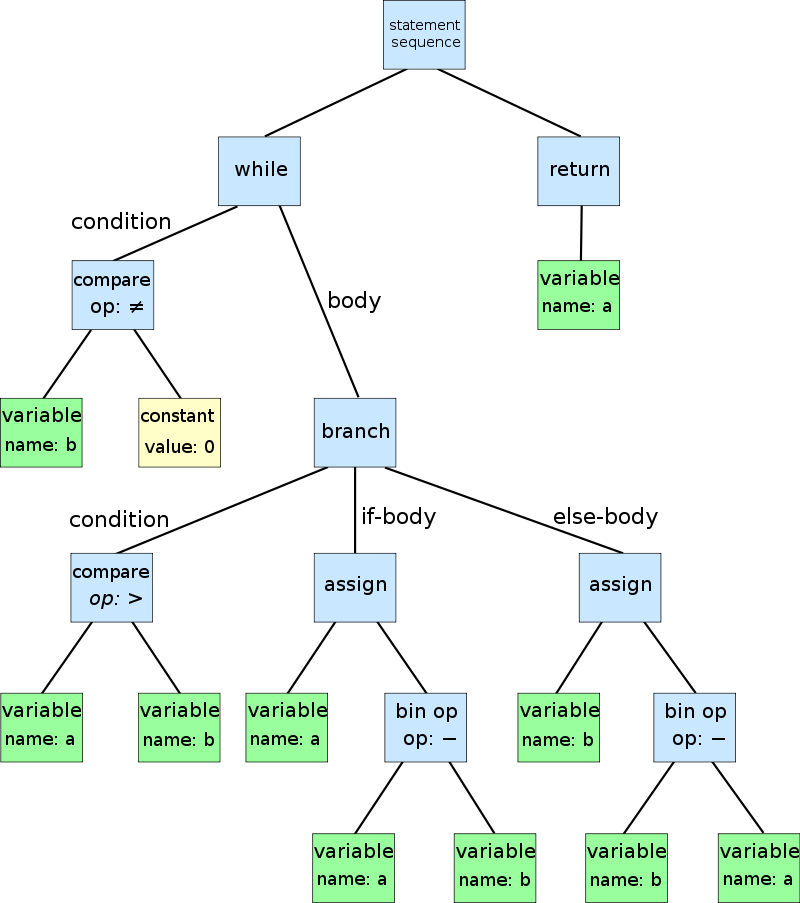
\includegraphics[width=0.75\textwidth]{figs/ast.png}
	\caption{Example of an AST for the Euclidean algorithm. Copied from \url{https://en.wikipedia.org/wiki/Abstract\_syntax\_tree}}
\end{figure}

\section{Implementation}
\label{sec:contract-implement}
Implementation of the Java 12 API caveat contract construction was completed purely using Python 3.6 and its standard libraries. The contracts generated were exported as a JSON array to be used in other applications (i.e. plugin) and can be found in the project repository (\url{./exception_range_rules_filtered.json}). The IntelliJ plugin was developed in Java 11.

\subsection{Java API Caveat Contracts}
\label{subsec:contract-caveat-contracts}
The JSON objects for caveats of the Java 12 classes were reused from \ref{subsec:info-caveat-extract} and loaded as a Pandas library \lstinline{DataFrame} object. The object consisted of rows of individual caveats while the columns represented various information about a caveat such as the sentence involved and which class it belonged to. This allowed filtering functions to be easily applied such that a subset of the caveats could be selected based on some condition. Constructing the caveat contracts involved following the algorithm described in \ref{subsec:contract-construct}. In particular, the regular expressions in \ref{tab:zhou-regex} and \ref{tab:normalisation-regex} were written in Python's \lstinline{re} library syntax. In addition to the algorithm described in \ref{subsec:contract-construct}, a simpler approach was also considered for \textit{not-null} caveats. From observation of the exception level sentences of the Java 12 documentation, it was found that any mention of the term ``null'' would usually imply an exception to be thrown if some parameter was \lstinline{null}. Therefore, an approach to capture all \textit{non-null} caveats for exception level sentences involves a sub-string check to see if ``null'' appears within the sentence. It was assumed that the same logic could be applied to the caveat categories of interest (\textit{range limitation} and \textit{type restriction}). Furthermore, it was noted that these caveat sentences would require certain key terms to be considered at all for a category (e.g. ``null'' would have to appear within a sentence to specify whether \lstinline{null} is allowed or not). 
Generalised regular expressions were then used to filter the caveat sentences into whether they potentially belonged to one of the caveat categories of interest. For example, to collect caveats that potentially issued a \textit{non-null} constraint, ``null'' was used as a search term and the sentence was considered if it contained the sub-string ``null''. The complete list of regular expressions used can be found in the \url{APIDoc2Rules.ipynb} Jupyter notebook. Applying these filters resulted in significantly smaller sets of caveat sentences that required manual labelling to determine what constraints they described for future contract construction. Specifically, the unique potential \textit{not-null} exception and parameter sentences totalled 835 and 193 respectively. For the \textit{range limitation} category, the exception and parameter sentences totalled 193 and 149 respectively. Given the small sets of sentences obtained, a random sample of size 100 was collected for each group/filter. For the \textit{not-null} categories of exception and parameter sentences, the subject parameter of the constraint was labelled. As an example, for the sentence ``prefix - the prefix of the tag, may not be null'', \textit{prefix} would be marked as the constraint subject. Note that the parameter sentences follow a template as described in \ref{subsec:contract-caveat-statistics} which makes extracting the relevant parameter trivial whereas for an exception sentence such as ``if the specified sorted set is null'' from the constructor of the \lstinline{java.util.TreeSet<E>} class, parsing is harder given that the name of the relevant parameter (``s'' in this case) is not used.

For the \textit{range limitation} sentences, the constraints were expressed as a mathematical expression. An example of this is with the sentence ``IllegalArgumentException - if iv is null or (iv.length - offset < 2 * (wordSize / 8))'' from the \lstinline{RC5ParameterSpec} constructor of the \lstinline{javax.crypto.spec.RC5ParameterSpec} class, the constraint of the sentence would be identified as $iv.length-offset<2*(wordSize/8)$. After manual labelling, 90\% of the 100 random parameter sentences filtered for \textit{not-null} were found to actually describe a \textit{not-null} constraint. For the exception level sentences, 87\% were found to describe a \textit{not-null} constraint. Moreoever, for the \textit{range-limitation} samples, 49\% and 72\% of the parameter and exception sentences were found to express an range limitation constraint, respectively. These results reveal that using basic sub-string searches for \textit{not-null} constraints is a viable approach for the Java 12 API documentation, while more complex approaches are required for identifying (and extracting) \textit{range limitation} caveats. Applying the sentence normalisation algorithm described in \ref{subsec:contract-construct}, the constraints were found to be correctly extracted for 41 of the 72 API caveat sentences with a range limitation constraint in the sample. An additional 13 caveat sentences were partially able to extract the correct constraints (which would also cause an exception to be thrown). Overall, the results are represented in terms of a confusion matrix in \ref{tab:conf-mat} to allow computation of accuracy, and F-measure. It can be seen that the true positive (TP) is 54, true negative (TN) is 25, false positive (FN) is 2, and the false negative is 19. Using the equations \ref{accuracy}, \ref{recall}, \ref{precision} and \ref{f-measure}, the accuracy is 0.77, recall is 0.73, precision is 0.96 and F1 score is 0.83. These results suggest that applying sentence normalisation is a viable approach for extracting constraints from sentences that describe exceptions thrown under certain conditions (or at least for the Java 12 API documentation). These extracted constraints were then used to represent API caveat contracts in static code analysis. Each caveat contract consisted of the full class name of the associated API caveat, the method name and its signature (containing its return type and list of parameters), and the constraint for one of the parameters. Overall, 4,694 unique contracts were constructed for the Java 12 API documentation using the sentence normalisation algorithm proposed (in regards to \textit{not-null} or \textit{range limitation} constraints).

\begin{table}[]
	\begin{tabular}{l|l|l|}
		\cline{2-3}
		& \textbf{Predicted Non-constraint} & \textbf{Predicted Constraint} \\ \hline
		\multicolumn{1}{|l|}{\textbf{Actual Non-constraint}} & 25 & 2 \\ \hline
		\multicolumn{1}{|l|}{\textbf{Actual Constraint}} & 19 & 54 \\ \hline
	\end{tabular}
	\caption{Confusion matrix for the sentence normalisation approach proposed.}
	\label{tab:conf-mat}
\end{table}

\begin{equation}
\label{accuracy}
\text{accuracy} = \frac{TP + TN}{TP + TN + FP + FN}
\end{equation}

\begin{equation}
\label{recall}
\text{recall}=\frac{TP}{TP + FN}
\end{equation}

\begin{equation}
\label{precision}
\text{precision}=\frac{TP}{TP + FP}
\end{equation}

\begin{equation}
\label{f-measure}
\text{F1}=\frac{2\cdot recall\cdot precision}{recall + precision}
\end{equation}

\subsection{IntelliJ Plugin with Static Code Analysis}
\label{subsec:contract-plugin}
IntelliJ's PSI provides the \lstinline{AbstractBaseJavaLocalInspectionTool} class that can be extended for creating plugins involving static code analysis. This was used to define a \textit{visitor} that would traverse the AST of a program periodically. In addition to this, classes were defined for the concepts of an API method, API class, caveat, and for storing a collection of all caveat contracts loaded from \ref{subsec:contract-caveat-contracts}. Java's \lstinline{HashMap} was used as the underlying data structure for storing the caveat contracts. This tree-like structure allowed searching for the contracts of an arbitrary method to consist of two simple steps: obtaining the methods attached to a certain class (via the full class name as a hash), finding the correct method by searching through the associated list of methods. It is noted that further optimisations could be used in the future to quicken the retrieval of contracts for a given API method such as using the hash of the method signature to map directly to its caveat contracts. However, a simple design was chosen given that the plugin was a proof-of-concept application. Overall, the code analysis process involved implementing the visit function for the visitor such that each expression call in the program would be analysed. Specifically, the full class name, method name and argument types would be identified. The caveat contracts associated to the API call would then be retrieved. Each caveat contract would then be invoked and checked given the argument values provided to the API call. For the \textit{not-null} constraints, this check simply required comparing the argument values to \lstinline{null}. For the \textit{range limitation} constraints, the logical operators ($<$, $\leq$, etc.) were also included alongside the comparing value in the contracts constructed from \ref{subsec:contract-caveat-contracts}. This meant that an SMT solver was not required and we could simply applying the range constraints in Java code, though an SMT solver could be used in future for more complex constraints. We also note here that as baseline checker program, we only analyse argument values passed directly to an API call. Furthermore, the caveat categories of interest for this thesis are \textit{not-null} and \textit{range limitation}, which do not require further analysis of a program's AST even though more complex analysis can be conducted (such as evaluating expressions/variables that are passed as arguments to an API call). IntelliJ's PSI then provides the functionality to register a problem that will be displayed within the code editor of the IDE. Each caveat contract that was found to be violated would then result in a problem to be registered for the associated API call.

\section{Results}
\label{sec:contract-results}
From the construction of caveat contracts for the Java 12 API documentation, and from the checker plugin implemented for IntelliJ, a proof-of-concept for applying natural language to source code was completed. To showcase an example of the plugin's functionalities, \ref{fig:plugin-inspection-off} illustrates several constraint-violating API calls for Java 12 API elements in IntelliJ. Using the plugin, the result is each constraint-violation is highlighted in IntelliJ with red squiggly lines as shown in \ref{fig:plugin-inspection-on}. Hovering the cursor over any of these highlighted problems will bring show a pop-up that provides more detailed information about the caveat contract violation. An example of this is shown in \ref{fig:plugin-problem}. In these examples, IntelliJ version 2018.2.4 (community edition) was used.

\begin{figure}
	\label{fig:plugin-inspection-off}
	\centering
	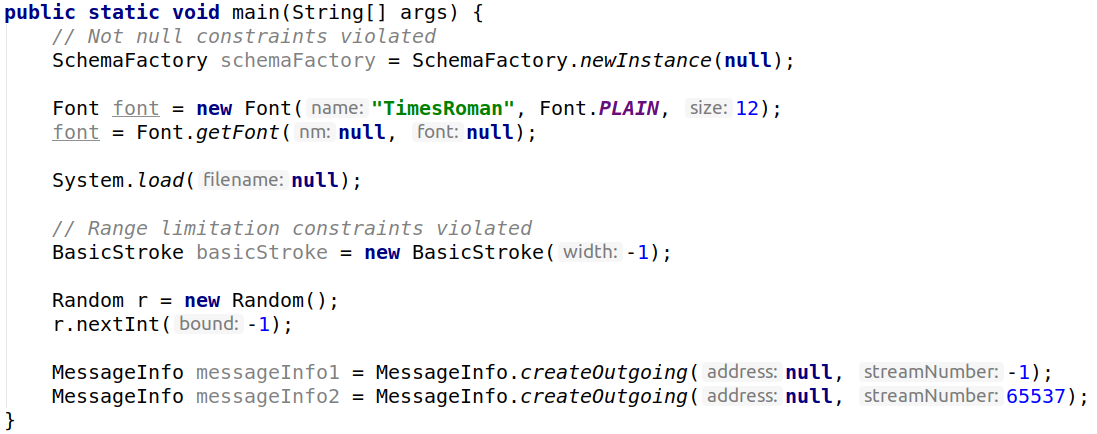
\includegraphics[width=0.85\textwidth]{figs/plugin-inspection-off.png}
	\caption{Example of IntelliJ's (lack of) problem highlights for obvious constraint violations.}
\end{figure}

\begin{figure}
	\label{fig:plugin-inspection-on}
	\centering
	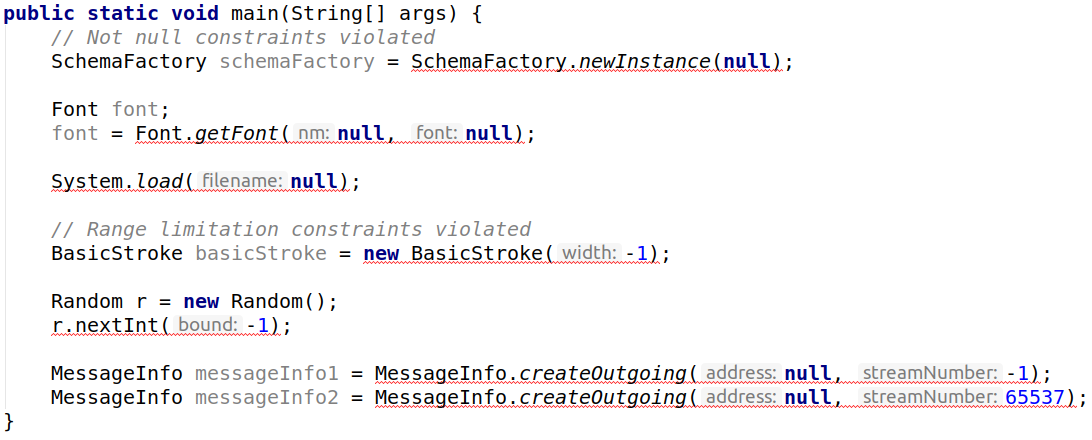
\includegraphics[width=0.85\textwidth]{figs/plugin-inspection-on.png}
	\caption{Example of how the developed plugin handles API caveat contract violations.}
\end{figure}

\begin{figure}
	\label{fig:plugin-problem}
	\centering
	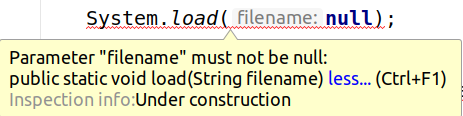
\includegraphics[width=0.3\textwidth]{figs/plugin-problem.png}
	\caption{Example of displayed problem message for an API caveat contract violation using the plugin.}
\end{figure}

It is noted that IntelliJ does implement its own version of contracts that require annotations following a specific syntax within the IDE. However, these contracts must be manually implemented for each method and were found to be mostly inconsistent. An example of this inconsistency is shown in \ref{fig:intellij-inspection-on} and \ref{fig:intellij-inspection-off}. In \ref{fig:intellij-inspection-on}, a \textit{not-null} constraint is violated for the \lstinline{isAfter} API call and correctly highlighted by IntelliJ's contracts. In \ref{fig:intellij-inspection-off}, another \textit{not-null} constraint is violated for the \lstinline{add} method of a \lstinline{PriorityQueue} object, which throws a \lstinline{NullPointerException} if executed. Hence, it can be seen that the code contracts implementation has two major drawbacks: it requires manual implementation of IntelliJ contracts for each method, and it is inconsistent (potentially as a result of the first problem). The plugin implemented is able to solve the first problem by automating the process of mapping sentences from the Java 12 API documentation to custom caveat contracts. Furthermore, it is able to solve the second problem with manual intervention as constraints for each individual API element are extracted and parsed into caveat contracts.

\begin{figure}
	\label{fig:intellij-inspection-on}
	\centering
	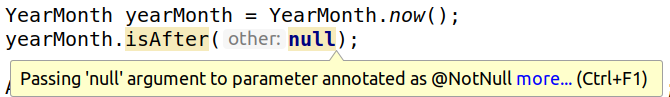
\includegraphics[width=0.5\textwidth]{figs/intellij-inspection-on.png}
	\caption{Example of IntelliJ's contracts.}
\end{figure}

Overall, the plugin in its current iteration is able to highlight the explicit contract violations from the Java 12 API documentation related to \textit{not-null} or \textit{range limitation} constraints. It is clear that with the addition of other categories of API caveats mapped to contracts, the plugin could be used to highlight many errors and problems for developers in real-time, which could minimise API misuse and help developers learn correct usage of an API. In terms of constructing caveat contracts, further research could yield methods that both improve the precision and recall of constraints extraction. It could also be used to bridge the gap between developers of an API and users of the given APIs such that API misuses can be minimised. In terms of static code analysis, the plugin shows that natural language can be applied to source code to improve understanding of an API, avoid API misuses and potentially increase efficiency of learning/development for programmers.

\begin{figure}
	\label{fig:intellij-inspection-off}
	\centering
	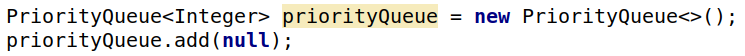
\includegraphics[width=0.5\textwidth]{figs/intellij-inspection-off.png}
	\caption{Example of IntelliJ's contract inconsistency.}
\end{figure}

\section{Summary}
\label{sec:contract-summary}
This chapter focused on the concept of code contracts and associated it to API caveats. The idea of transforming API caveats to contracts was presented and implemented for a subset of API caveats that were related to \textit{not-null} and \textit{range limitation} constraints. A statistical analysis was also performed to determine the prevalence of these categories of caveats in the Java 12 API documentation. It was found that 20\% of unique API caveat sentences appearing in the exception sections of the documentation imposed a \textit{not-null} constraint. For the \textit{range limitation} category, 13\% of unique API caveat sentences were found to describe a constraint involving range. These categories were chosen for investigation and implementation of code contracts as they were explicit constraints that would result in an exception and could be considered the baseline API caveats for mapping natural language to code contracts. Furthermore, a sentence normalisation algorithm was proposed for extracting the range constraints from sentences and used to construct 4,694 unique contracts. Design and implementation of a proof-of-concept IntelliJ plugin that acted as checker for the the caveat contracts was also presented. The potential of this approach for linking natural language to source code was also discussed. In particular, the plugin showcases that API misuses could be detected in real-time, improve understanding of APIs and direct developers to correct usage of an API.\\
In Chapter \ref{cha:conc}, the findings of this thesis are summarised and ideas for future work are presented. Lastly, some final remarks about the research focus of this thesis are expressed.
